%************************************************
\chapter{Cálculo de la homología singular}\label{ch:calculoI}
%************************************************

En esta parte, vamos a enunciar y demostrar el teorema de subdivisión baricéntrica,
el cual nos permite calcular directa o indirectamente (a través de sus consecuencias)
los grupos de homología de ciertos espacios topológicos, como haremos con las esferas
n-dimensionales.

\section{Teorema de subdivisión baricéntrica}

\begin{definition}
  Sea $\X$ un espacio topológico. Diremos que $\U \subseteq \mathcal P(\X)$ es un recubrimiento de $\X$ si $\X = \bigcup\limits_{U \in \U} U$.
\end{definition}

Tomemos ahora $\X$ un espacio topológico y $\U$ un recubrimiento suyo. Para $ p \geq 0$, podemos definir:
\[ F_p^\U(\X) = \{\phi \in F_p(\X) \mid \exists U \in \U \text{ tal que } \Img \phi \subseteq U\} \]
que es, por definición, subconjunto de $F_p(\X)$.

Si $S_p^\U(\X)$ es el grupo abeliano libre generado por $F_p^\U(\X)$, por $F_p^\U(\X) \subseteq F_p(\X)$, se tiene
que $S_p^\U(\X)$ es un subgrupo de $S_p(\X)$. Si consideramos la inclusión $i \colon S_p^\U(\X) \to S_p(\X)$, si
$\phi \in F_p^\U(\X)$, entonces $\partial_i(\phi) \in F_{p-1}^\U(\X)$ y así, por la definición del borde, $\partial(\phi) \in S_{p-1}^\U(\X)$. \\
En consecuencia, la restricción del borde a $S_p^\U(\X)$ define un homomorfismo borde, y así, construímos un complejo
de cadenas $S_*^\U(\X) = \{S_p^\U(\X), \partial\}_{p \geq 0}$.

Es claro que este complejo es un subcomplejo de $S_*(\X)$. Si tomamos la inclusión $i \colon S_*^\U(\X) \to S_*(\X)$, induce un
homomorfismo en la homología, $i_* \colon H_p(S_*^\U(\X)) \to H_p(\X) \hspace{0.2em} \forall p \geq 0$, donde
$H_p(S_*^\U(\X)) = \frac{\Ker \partial}{\Img \partial}$, con el borde actuando en $S_*^\U(\X)$.

Sea ahora $\Y$ otro espacio topológico, y $\V$ un recubrimiento suyo. Diremos que una función continua $f \colon \X \to \Y$ es compatible
con $\U, \V$ si $\forall U \in \U \hspace{0.5em} \exists V \in \V$ tal que $f(U) \subseteq V$. En tal caso, puede definirse
$f_\# \colon S_p^\U(\X) \to S_p^\V(\Y)$, homomorfismo, dado por la restricción de $f_\# \colon \SX{p} \to \SY{p}$ a $S_p^\U(\X)$.

Esto hace que el siguiente diagrama sea conmutativo:
\[ \begin{tikzcd}
  S_p^\U(\X) \arrow{r}{f_\#} \arrow{d}{i} & S_p^\V(\Y) \arrow{d}{i} \\
  \SX{p} \arrow{r}{f_\#} & \SY{p}
\end{tikzcd} \]

\begin{remark}
  El diagrama conmutativo está bien definido, pues si $\phi \in F_p^\U(\X)$, entonces existe $U \in \U$ con $\Img \phi \subseteq U$, de donde
  $f_\#(\phi) = f \circ \phi$ verifica $\Img(f \circ \phi) \subseteq f(U) \subseteq V \in \V$.
\end{remark}

Como $f_\# \partial = \partial f_\#$, $f$ induce $f_* \colon H_p(S_p^\U(\X)) \to H_p(S_p^\V(\Y))$.

Nos encontramos en condiciones de enunciar el teorema de subdivisión baricéntrica, que relaciona complejo de cadenas
de un espacio con un recubrimiento con el complejo de cadenas del espacio.

\begin{theorem}[Teorema de subdivisión baricéntrica]
  Sean $\X$ un espacio topológico y $\U$ un recubrimiento de $\X$ tal que $\interior{\U} = \{\interior{U} \mid U \in \U\}$
  también recubra a $\X$. Entonces la aplicación
  \[ i_* \colon H_p(S_*^\U(\X)) \to H_p(\X) \]
  es un isomorfismo, $\forall p \geq 0$.

  Además, si $(\Y, \V)$ es otro par de las mismas características, y $f \colon \X \to \Y$ es una función continua
  compatible con $\U, \V$, entonces el siguiente diagrama es conmutativo:
  \[ \begin{tikzcd}
    H_p(S_*^\U(\X)) \arrow{r}{i_*} \arrow{d}{f_*} & H_p(\X) \arrow{d}{f_*} \\
    H_p(S_*^\V(\Y)) \arrow{r}{i_*} & H_p(\Y)
  \end{tikzcd} \]

\end{theorem}

Antes de pasar a la demostración del teorema, necesitaremos introducir nuevos conceptos. La idea es definir la subdivisión
de símplices singulares mediante la subdivisión baricéntrica de símplices, que nos llevan a poder dar una especie de
inversa homotópica de la inclusión.

\section{Subdivisión de símplices}

Vamos a definir la subdivisión baricéntrica de símplices, utilizando nociones geométricas.

\begin{definition}
  Sea $s_p = (a_0, \dots, a_p)$ un p-símplice. Definimos el baricentro de $s_p$ como
  \[b(s_p) = \frac{a_0 + \dots + a_p}{p+1}\]
\end{definition}

Los puntos $\{b(s_p), a_0, \dots, a_{i-1}, a_{i+1}, \dots, a_p\}$ genera un p-símplice $\forall i = 0, \dots, p$.
Definimos la subdivisión baricéntrica del símplice $s_p$ por inducción sobre $p$, y la notamos $Sd(s_p)$.
\begin{itemize}
  \item $Sd(s_0) = s_0$
  \item $Sd(s_p) = (b(s_p), t_0, \dots, t_{p-1}) \mid (t_0, \dots, t_{p-1}) \in Sd(\U_{p-1}), \U_{p-1} \in \interior{S_p}$
        siendo $\interior{S_p}$ el conjunto de caras de orden $p-1$ de $S_p$.
\end{itemize}

\begin{remark}
  Es importante destacar que el orden en el que se ponen los puntos es importante, pues si el baricentro fuera en otro lugar,
  la orientación del símplice cambiaría, y afectaría al cálculo del borde.
\end{remark}

\begin{example}
  Vemos una representación gráfica de la subdivisión baricéntrica.

  \begin{tikzpicture}
    baseline=(current bounding box.center)
    \draw [] (0, 0) circle (2pt) -- (2, 2) circle (2pt);
  \end{tikzpicture}
  $\rightarrow{\makebox[2cm]{}}$
  \begin{tikzpicture}
    baseline=(current bounding box.center)
    \draw [] (0, 0) circle (2pt) -- (1, 1) circle (2pt) -- (2, 2) circle (2pt);
  \end{tikzpicture}

  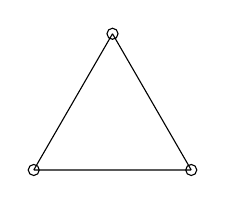
\begin{tikzpicture}
    baseline=(current bounding box.center)
    \draw [] (0, 1.73) circle (2pt) -- (1, 0) circle (2pt) -- (-1, 0) circle (2pt) -- (0, 1.73);
  \end{tikzpicture}
  $\rightarrow{\makebox[2cm]{}}$
  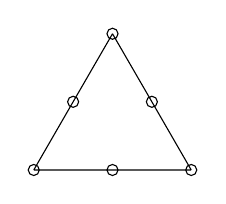
\begin{tikzpicture}
    baseline=(current bounding box.center)
    \draw [] (0, 1.73) circle (2pt) -- (0.5, 0.866) circle (2pt) -- (1, 0) circle (2pt) -- (0, 0) circle (2pt) --
    (-1, 0) circle (2pt) -- (-0.5, 0.866) circle (2pt) -- (0, 1.73);
  \end{tikzpicture}
  $\rightarrow{\makebox[2cm]{}}$
  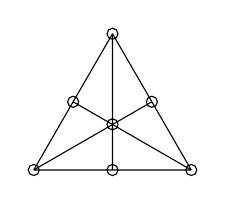
\begin{tikzpicture}
    baseline=(current bounding box.center)
    \draw [] (0, 1.73) circle (2pt) -- (0.5, 0.866) circle (2pt) -- (1, 0) circle (2pt) -- (0, 0) circle (2pt) --
    (-1, 0) circle (2pt) -- (-0.5, 0.866) circle (2pt) -- (0, 1.73);
    \draw [] (0.5, 0.866) -- (-1, 0);
    \draw [] (-0.5, 0.866) -- (1, 0);
    \draw [] (0, 0) -- (0, 0.58) circle (2pt) -- (0, 1.73);
  \end{tikzpicture}
\end{example}

Si $K$ es un conjunto de símplices, la subdivisión de $K$ vienen dada por $Sd(K) = \bigcup\limits_{s_p \in K} Sd(s_p)$.

Se define la n-ésima subdivisión como \[Sd^n(s_p) = Sd(Sd^{n-1}(s_p)), \text{ con } Sd^1 = Sd \]

\begin{proposition}
  Sea $t_p \in Sd(s_p)$ un p-símplice de la subdivisión. Entonces $diam(t_p) \leq \frac{p}{p+1} diam(s_p)$.
\end{proposition}

\begin{proof}
  Haremos la demostración por inducción sobre $p$.

  Para $p = 0$, se tiene $0 = 0$.

  Supuesto cierto hasta $p-1$, lo probamos para $p$.

  Sea $s_p = (a_0, \dots, a_p)$. Se verifica que $diam(s_p) = \max\limits_{i,j} |a_i - a_j|$.
  Como $t_p \in Sd(s_p), t_p = (b(s_p), t_0, \dots, t_{p-1}) \in Sd(\U_{p-1})$.
  Entonces, $diam(t_p) = max\{|b(s_p) - t_i|,\hspace{0.2em} |t_i - t_j|, i,j = 0, \dots, p-1\}$.

  Por h. de inducción sabemos que $|t_i - t_j| \leq diam(t_0, \dots, t_{p-1}) \leq \frac{p-1}{p} diam(\U_{p-1})$.
  Como $U_{p-1} \subseteq s_p$, entonces $diam(U_{p-1}) \leq diam(s_p)$, y como $\frac{p-1}{p} \leq \frac{p}{p+1}$
  se tiene $|t_i - t_j| \leq \frac{p}{p+1} diam(s_p)$

  Además, $|b(s_p) - t_i| \leq \max\limits_i |b(s_p) - a_i| = \max\limits_i |\frac{a_0 + \dots + a_p}{p-1} - a_i| =
  \max\limits_i | \frac{\sum\limits_{i \neq j} |a_j - a_i|}{p+1} \leq \frac{p}{p+1} diam(s_p)$
\end{proof}

\begin{definition}
  Sea $\varphi$ una colección de subconjuntos acotados de un espacio euclídeo. Definimos $malla \varphi = \sup\limits{c \in \varphi} diam(c)$
\end{definition}

\begin{corollary}
  Si $K$ es una colección de p-símplices, se verifica \[malla(Sd(K)) \leq \frac{p}{p+1} malla(K) \]
\end{corollary}

\begin{corollary}
  Si $K$ es una colección finita de p-símplices, entonces $\forall \epsilon > 0, \exists n \in \N$ tal que \\$malla(Sd^n(k)) < \epsilon$
\end{corollary}

\begin{proof}
  Simplemente aplicamos $\lim\limits_{n \to \infty}(\frac{p}{p+1})^n = 0$
\end{proof}

\section{Subdivisión baricéntrica de símplices singulares afines}

Vamos a tratar ahora la subdivisión de símplices singulares afines. Estos nos permitirán aproximar la
subdivisión de cualquier símplice singular, por lo que su estudio nos resulta de gran interés.

Sea $C$ un subconjunto convexo del espacio euclídoe en el que trabajamos. Para todo $p \geq 0$, sea
\[F_p^A(C) = \{ \phi \in F_p(C) \mid \phi \text{ es una aplicación afín}\} \]
es decir, $\phi \colon \sigma_p \to C \quad$ verifica \[\phi(ta + (1-t)b) = t\phi(a) + (1-t)\phi(b) \hspace{1em} \forall t \in [0,1]\]

Sea $A_p(C)$ el grupo abeliano libre generado por $F_p^A(C)$, subgrupo libre de $S_p(C)$. Si $\phi \in F_p^A(C), \partial_i \phi = \phi \circ F_p^i$,
y como $\phi$ es afín y $F_p^i$ también, $\partial_i \phi$ es afín. Así:
\[\partial \phi = \sum\limits_{i = 0}^p (-1)^1 \partial_i \phi \hspace{0.5em} \in A_{p-1}(C)\]

Es consecuencia, podemos restringir el borde a $A_p(C)$, haciendo conmutativo
\[ \begin{tikzcd}
      A_p(C) \arrow{r}{\partial} \arrow{d}{i} & A_{p-1}(C) \arrow{d}{i} \\
      S_p(C) \arrow{r}{\partial} & S_{p-1}(C)
\end{tikzcd} \]

Tenemos pues un complejo de cadenas $A_*(C) = \{A_p(C), \partial\}_{p \geq 0}$, para todo convexo $C$.

Si $\phi \in F_p^A(C), \phi \colon \sigma_p \to C$ afín. Notando $\sigma_p = (v_0, \dots, v_p)$, entonces
${x_i = \phi(v_i) \in C}$ determinan unívocamente a $\phi$, pues si $v = \sum\limits_{i = 0}^p \alpha_i v_i$, entonces
$\phi(v) = \sum\limits_{i = 0}^p \alpha_i \phi(v_i)$ por afinidad. Por tanto, todo elemento de $\phi \in F_p^A(C)$ se
identifica con $p+1$ puntos de $C$.
\[\phi \in F_p^A(C) \equiv \{x_0, \dots, x_p\} \subseteq C\]

Además, $\partial \phi = \sum\limits_{i = 0}^p (-1)^i \partial_i \phi$, con $\partial_i \phi = \{x_0, \dots, \hat{x_i}, \dots, x_p\}$

En consecuencia, $A_p(C)$ es el grupo abeliano libre sobre:
\[\{(x_0, \dots, x_p) \mid x_i \in C\} \equiv C \times \dots \times C \]
y el operador borde lo da $\partial(\{x_0, \dots, x_p\}) = \sum\limits_{i = 0}^p (-1)^i \{x_0, \dots, \hat{x_i}, \dots, x_p\}$

Si tenemos $C, C'$ convexos, y $f \colon C \to C'$ es una aplicación afín (y por tanto continua), al tomar la restricción de $f_\#$
a $A_p(C)$, se tiene que si ${\phi \in F_p^A(C)}$ entonces $f_\#(\phi) = {f \circ \phi \in F_p^A(C')} \implies {f_\#(A_p(C)) \subseteq A_p(C')}$

En consecuencia, $\partial f_\# = f_\# \partial$ y $f_\# \colon A_*(C) \to A_*(C')$ es una aplicación de cadenas. Además,
${f_\#(\{x_0, \dots, x_p\}) = \{f(x_0), \dots, f(x_p)\}}$

\begin{definition}
  Sea $x \in C$ Definimos
  \begin{align*}
    \C_x \colon A_p(C) &\to A_{p+1}(C) \\
    \{x_0, \dots, x_p\} &\mapsto \{x, x_0, \dots, x_p\}
  \end{align*}
  y la extendemos por linealidad a un homomorfismo, pues tenemos los valores de los generadores.
\end{definition}

\begin{proposition}
  Veamos que:
  \begin{itemize}
    \item[a)] $\partial \C_x + \C_x \partial = Id_{A_p(C)} \quad \forall p \geq 1$
    \item[b)] $f_\# \C_x = \C_{f(x)} f_\# \quad \forall f \colon C \to C'$ afín.
  \end{itemize}
\end{proposition}

\begin{proof}
  a) $\partial \C_x(x_0, \dots, x_p) = \partial(x, x_0, \dots, x_p) = \{x_0, \dots, x_p\} + \\ \sum\limits_{i = 1}^{p+1} (-1)^i \partial_i (x, x_0, \dots, x_p)
  = \{x_0, \dots, x_p\} + \sum\limits_{j = 0}^{p} (-1)^{j+1} \partial_{j+1} (x, x_0, \dots, x_p)
  = \{x_0, \dots, x_p\} - \sum\limits_{j = 0}^{p} (-1)^j \C_x(x_0, \dots, \hat{x_j}, \dots, x_p) = \{x_0, \dots, x_p\} - \C_x \partial(x_0, \dots, x_p)$

  b) $f_\# \C_x(x_0, \dots, x_p) = f_\#(x, x_0, \dots, x_p) = (f(x), f(x_0), \dots, f(x_p)) = \C_{f(x)} f_\#(x_0, \dots, x_p)$
\end{proof}

Ahora podemos definir una subdivisión para símplices o cadenas afines. Lo haremos por inducción, definiendo ${Sd' \colon A_p(C) \to A_p(C)}$

$\fbox{p = 0}$
\[Sd' = Id_{A_p(C)}\]

$\fbox{p > 0}$, supuesto definido hasta $p-1$
\[ Sd'(\phi) = \C_{b(\phi)}(Sd' \circ \partial \phi) \]
donde $b(\phi) = \frac{x_0 + \dots + x_p}{p+1}$, siendo $\phi = \{x_0, \dots, x_p\}$ y extendido linealmente.

Veamos algunas propiedades. Debido a que la definición se hizo por inducción, todas las demostraciones serán por inducción.

a) $\partial \circ Sd' = Sd' \circ \partial$

\begin{proof}
  Para $p = 0$ la demostración es trivial, por la definición de $Sd'$. Suponemos $p \geq 1$.

  Sea $\phi \in F_p^A(C)$, entonces
  \begin{align*}
    \partial \circ Sd'(\phi) &= \partial \C_{b(\phi)} Sd' \partial \phi = Sd'(\partial \phi) - \C_{b(\phi)} \partial Sd'(\partial \phi) \\
    &= Sd'(\partial \phi) - \C_{b(\phi)} Sd'(\partial^2 \phi) = Sd'(\partial \phi)
  \end{align*}
\end{proof}

b) Si $f \colon C \to C'$ es afín, entonces $f_\# \circ Sd' = Sd' \circ f_\#$

\begin{proof}
  $(f_\# Sd')(\phi) = f_\#(\C_{b(\phi)} Sd'(\partial(\phi))) = \C_{f(b(\phi))} f_\# Sd'(\partial(\phi))\\ \stackrel{\text{h. de i}}{=}
  \C_{f(b(\phi))} Sd'(f_\#(\partial(\phi))) = \C_{f(b(\phi))} Sd'(\partial(f_\#(\phi))) = Sd'(f_\#(\phi))$
\end{proof}

c) Existe un homomorfismo $\tau' \colon A_p(C) \to A_{p+1}(C)$ tal que ${\partial \tau' + \tau' \partial = Sd' - Id_{A_p(C)}}$,
es decir, $Sd'$ es, como aplicación de cadenas, homotópica a la identidad.

\begin{proof}
  Para $p = 0$, tomamos $\tau' = 0$

  Supuesto cierto hasta $p-1$, buscamos $\tau' \colon A_p(C) \to A_{p+1}(C)$ verificando
  \[\partial \tau' = Sd' - I_{A_p(C)} - \tau' \partial\]

  Como el segundo miembro es conocido, entonces si $\phi \in F_p^A(C), \tau'(\phi)$ ha de verificar
  \[\partial(\tau'(\phi)) = Sd'(\phi) - \phi - \tau'(\partial(\phi))\]
  lo calculamos
  \begin{align*}
    &\partial(Sd'(\phi) - \phi - \tau'(\partial(\phi)) = Sd'(\partial(\phi)) - \partial(\phi) - \partial(\tau' \partial(\phi)) \\
    &= Sd'(\partial(\phi)) - \partial(\phi) + \tau'(\partial^2(\phi)) - Sd'(\partial(\phi)) + \partial(\phi) = 0
  \end{align*}
  Definiendo $\tau'(\phi) = \C_{b(\phi)}(Sd'(\phi) - \phi - \tau'(\partial(\phi))$, entonces
  \begin{align*}
    &\partial(\tau'(\phi)) = \partial \C_{b(\phi)}(Sd'(\phi) - \phi -\tau'(\partial(\phi))) = (Sd'(\phi) - \phi - \tau' \partial(\phi)) \\
    &- \C_{b(\phi)} \partial(Sd'(\phi) - \phi - \tau'(\partial(\phi))) = Sd'(\phi) - \phi - \tau'(\partial(\phi))
  \end{align*}
\end{proof}

d) $\tau'$ es natural, esto es, si $f \colon C \to C'$ es afín, entonces $f_\# \tau' = \tau' f_\#$

\begin{proof}
  Para $p = 0$ es trivial por definición.

  Suponemos cierto hasta $p-1$. Sea $\phi \in F_p^A(C)$, entonces
  \begin{align*}
    &f_\#(\tau'(\phi)) = f_\#(\C_{b(\phi)}(Sd'(\phi) - \phi - \tau'(\partial(\phi))) \\
    &= \C_{f(b(\phi))} f_\#(Sd'(\phi) - \phi - \tau(\partial(\phi))) \\
    &= \C_{f(b(\phi))}(Sd'(f_\# \phi) - f_\# \phi - \tau'(f_\# \partial(\phi))) = \tau'(f_\#(\phi))
  \end{align*}
\end{proof}

e) Propiedad técnica. Nos permitirá subdividir símplices hasta que estos queden dentro del recubrimiento.

Sea $c = \sigma_p$ y $\tau_p \colon \sigma_p \to \sigma_p$ la identidad ($\tau_p \in F_p^A(\sigma_p)$). \\
Si $Sd'(\tau_p) = \sum_i n_i \phi_i$ (que ocurre siempre), con $\phi_i \colon \sigma_p \to \sigma_p$ afines, entonces
$\forall i \hspace{0.3em} \exists t_p^i \in Sd(\sigma_p)$ tal que $\Img(\phi_i) \subseteq t_p^i$.

\begin{proof}
  Para $p = 0$, $Sd'(\tau_0) = \tau_0 = \sigma_0$. Siendo $t_0^i = \sigma_0 = Sd'(\sigma_0)$.

  Supuesto cierto hasta $p-1$, sea $Sd'(\tau_p) = \C_{b(\tau_p)} Sd'(\partial(\tau_p))$
  \begin{align*}
    &\partial(\tau_p) = \sum\limits_{i = 0}^p (-1)^i \partial_i(\tau_p) = \sum\limits_{i = 0}^p (-1)^i \tau_p \circ F_p^i = (por ser la identidad) \\
    &= \sum\limits_{i = 0}^p (-1)^i F_p^i \circ \tau_{p-1} = \sum\limits_{i = 0}^p (-1)^i(F_p^i)_\# (\tau_{p-1}) \text{. De esta forma:} \\
    &Sd'(\tau_p) = \C_{b(\tau_p)}(\sum\limits_{i = 0}^p (-1)^i Sd'(F_p^i)_\# (\tau_{p-1})) = \C_{b(\tau_p)}(\sum\limits_{i = 0}^p (-1)^i(F_p^i)_\# Sd'(\tau_{p-1})) \\
  \end{align*}
  Si $Sd'(\tau_{p-1}) = \sum\limits_j m_j \psi_j$, entonces, por inducción, $\forall j$ existe $t_{p-1}^j \in Sd(\sigma_{p-1})$ tal que
  $\Img(\psi_j) \subseteq t_{p-1}^j$.

  Por tanto, $Sd'(\tau_p) = \sum\limits_{i = 0}^p \sum\limits_j (-1)^i m_j C_{b(\tau_p)}(F_p^i)_\# (\psi_j)$

  Como $\Img(\psi_j) \subseteq t_{p-1}^j \in Sd(\sigma_{p-1})$
  $\Img((F_p^i)_\# (\psi_j)) = \Img(F_p^i \circ \psi_j) \subseteq F_p^i(\Img(\psi_j)) \subseteq F_p^i(t_{p-1}^j) \in Sd(\interior{\sigma_p})$,
  luego $\Img((F_p^i)_\# (\psi_j)) \subseteq U_{p-1}^{i,j} \in Sd(\interior{\sigma_p})$.

  Así, $\Img(\C_{b(\tau_p)}(F_p^i)_\# (\phi_j)) \subseteq \C_{b(\tau_p)}(U_{p-1}^{i, j}) = (b(\sigma_p), t_0, \dots, t_{p-1}) \in Sd(\sigma_p)$.\\
  (Donde $U_{p-1}^{i,j} = (t_0, \dots, t_p)$)
\end{proof}

\section{Subdivisión de símplices singulares}

% Introducción

Nos basaremos en el caso afín.

\begin{proposition}
  Sea $\X$ un espacio topológico. Entonces, para todo $p \geq 0$ existe
  \[Sd\colon S_p{\X} \to S_p{\X} \] homomorfismo, verificando:
  \begin{itemize}
    \item[a)] Si $\X$ es un convexo de un espacio euclídeo, $\frac{Sd}{A_p(C)} = Sd'$
    \item[b)] $Sd \circ \partial = \partial \circ Sd$
    \item[c)] $Sd \circ f_\# = f_\# \circ Sd \quad \forall f \colon \X \to \Y$ continua
    \item[d)] Existe un homomorfismo $\tau \colon \SX{p} \to S_{p+1}(\X)$ tal que ${\partial \tau + \tau \partial = Sd - Id_{S_p(\X)}}$
              $\forall p \geq 0$ y $\tau f_\# = f_\# \tau \quad \forall f \colon \X \to \Y$ continua
    \item[e)] Si $\phi \in F_p(\X)$ y $Sd(\phi) = \sum_i n_i \phi_i$, entonces $\forall i \exists t_p^i \in Sd(\sigma_p)$ tal que
              $\Img(\phi_i) \subseteq \phi(t_p^i)$

  \end{itemize}
\end{proposition}

\begin{proof}
  Sea $\phi \in F_p(\X)$. Entonces, si $\tau_p \colon \sigma_p \to sigma_p$ es el p-símplice identidad, se tiene que
  $\phi = \phi_\#(\tau_p)$. En consecuencia, $Sd(\phi)$ debe verificar $Sd(\phi_\#)(\tau_p) = \phi_\#(Sd(\tau_p)) = \phi_\# Sd'(\tau_p)$. \\
  Definimos $Sd(\phi) = \phi_\#(Sd'(\tau_p))$ y lo extendemos por linealidad.

  Veamos ahora las propiedades.

  a) Si $\X$ es convexo, $\phi \in F_p^A(\X)$, y entonces, $Sd(\phi) = \phi_\# Sd'(\tau_p) = (Sd' \circ \phi_\#)(\tau_p) = Sd'(\phi)$
  pues ya lo hemos probado en este caso.

  b) \begin{align*}
    &(\partial \circ Sd)(\phi) = \partial \phi_\# Sd'(\tau_p) = \phi_\# \partial Sd'(\tau_p) = \phi_\# Sd'(\partial \tau_p) \\
    &= \phi_\#(Sd'(\sum\limits_{i = 0}^p (-1)^i (F_p^i)_\# (\tau_{p-1}))) = \phi_\#(\sum\limits{i = 0}^p (-1)^i Sd' \circ (F_p^i)_\#(\tau_{p-1}))\\
    &= \text{(caso afín)} = \phi_\#(\sum\limits_{i = 0}^p (-1)^i (F_p^i)_\# Sd'(\tau_{p-1})) = \sum\limits_{i = 0}^p (-1)^i (\phi \circ F_p^i)_\# Sd'(\tau_{p-1}) \\
    &= (\partial_i \phi)_\# (\sum\limits_{i = 0}^p (-1)^i Sd'(\tau_{p-1})) = \sum\limits_{i = 0}^p (-1)^i Sd(\partial_i \phi) = Sd(\sum\limits_{i = 0}^p (-1)^i \partial_i \phi) \\
    &= (Sd \circ \partial)(\phi)
  \end{align*}

  c) $(f_\# \circ Sd)(\phi) = f_\# \phi_\# Sd'(\tau_p) = (f \circ \phi)_\# Sd'(\tau_p) = Sd(f_\#(\phi))$

  d) Definimos \[\tau(\phi) = \phi_\#(\tau'(\tau_p)) \quad \text{con} \quad \phi_\# \colon S_{p+1}(\sigma_p) \to S_{p+1}(\X) \]
  Entonces, se tiene:
  \begin{align*}
    &(\partial \tau + \tau \partial)(\phi) \partial(\phi_\# \tau'(\tau_p)) + \tau(\sum\limits_{i = 0}^p (-1)^i \partial_i \phi) \\
    &= \phi_\#(\partial \tau'(\tau_p)) + \sum\limits_{i = 0}^p (-1)^i((\partial_i \phi)_\#(\tau'(\tau_{p-1})) = \phi_\#(\partial \tau'(\tau_p)) \\
    &+ \phi_\#(\sum\limits_{i = 0}^p (-1)^i (F_p^i)_\# (\tau'(\tau_{p-1}))) = \text{caso afín} = \phi_\#(\partial \tau'(\tau_p)) \\
    &+ \phi_\#(\tau'(\sum\limits_{i = 0}^p (-1)^i (F_p^i)_\#(\tau_{p-1})) = \phi_\#(\partial \tau'(\tau_p)) + \phi_\#(\tau'\partial(\tau_p)) \\
    &= \phi_\#(\partial \tau' + \tau' \partial)(\tau_p) = \text{caso afín} = \phi_\#(Sd' - Id)(\tau_p) = Sd(\phi) - \phi
  \end{align*}

  e) Como $Sd(\phi) = \phi_\#(Sd'(\tau_p))$, entonces si $Sd'(\tau_p) = \sum_i n_i \psi_i, \phi_i = \phi_\#(\psi_i)$

  Como existe $t_p^i \in Sd(\sigma_p)$ tal que $\Img(\psi_i) \subseteq t_p^i$, entonces
  \[\Img(\phi_i) = \Img(\phi_\#(\psi_i)) = \phi(\Img(\psi_i)) \subseteq \phi(t_p^i)\]

  \begin{remark}
    Probar que si $\phi \in F_p(\X)$ y $Sd^n(\phi) = \sum_i n_i \phi_i \implies \forall i \exists t_p^i \in Sd^n(\sigma_p)$ tal que
    $\Img(\phi_i) \subseteq \phi(t_p^i)$, consiste en reiterar la propiedad e) ya demostrada.
  \end{remark}

\end{proof}

\section{Demostración del teorema}

Demostremos ya el teorema de subdivisión baricéntrica. Recordamos su enunciado.

\begin{theorem}[Teorema de subdivisión baricéntrica]
  Sean $\X$ un espacio topológico y $\U$ un recubrimiento de $\X$ tal que $\interior{\U} = \{\interior{U} \mid U \in \U\}$
  también recubra a $\X$. Entonces la aplicación
  \[ i_* \colon H_p(S_*^\U(\X)) \to H_p(\X) \]
  es un isomorfismo, $\forall p \geq 0$.

  Además, si $(\Y, \V)$ es otro par de las mismas características, y $f \colon \X \to \Y$ es una función continua
  compatible con $\U, \V$, entonces el diagrama que obtenemos considerando $f_* e i_*$ es conmutativo.
\end{theorem}

\begin{proof}
  Sea $\X$ un espacio topológico, y sea $\U$ un recubrimiento de $\X$ tal que $\interior{\U}$ tambień recubre a $\X$.

  Si $\phi \in F_p(\X)$, esto es, $\phi \colon \sigma_p \to \X$ es continua, sea $V = \{\phi^{-1}(U) \mid U \in \U\}$, recubrimiento
  abierto de $\sigma_p$ como espacio métrico compacto. Sea $\epsilon(\phi)$ el número de Lebesgue de dicho recubrimiento.
  Así, si $A \subseteq \sigma_p$ y $diam(A) < \epsilon(\phi)$ entonces existe $U \in \U$ tal que $A \subseteq \phi^{-1}(U)$ y entonces
  $\phi(A) \subseteq U$

  En consecuencia, $\forall \phi \in F_p(\X) \quad \exists \epsilon(\phi) > 0$ tal que si $A \subseteq \sigma_p, diam(A) < \epsilon(\phi)$,
  entonces existe $U \in \U$ tal que $\phi(A) \subseteq(U)$

  Por un corolario que ya hemos visto, dado $\epsilon(\phi)$, existe $n(\phi)$ tal que \\
  ${malla(Sd^{n(\phi)}(\sigma_p)) < \epsilon(\phi)}$. Si $t_p \in Sd^{n(\phi)}(\sigma_p), diam(t_p) < \epsilon(\phi)$,
  luego existe $U \in \U$ con $\phi(t_p) \subseteq U$. En consecuencia, si $Sd^{n(\phi)}(\phi) = \sum_i n_i \phi_i$,
  entonces $\Img(\phi_i) \subseteq \phi(t_p^i)$ con $t_p^i \in Sd^{n(\phi)}(\sigma_p)$,
  por lo que existirá $U_i \in \U$ con $\Img(\phi_i) \subseteq \phi(t_p^i) \subseteq U_i$ \\
  Así, $Sd^{n(\phi)}(\phi) \in S_p^\U(\X)$

  Sea $m(\phi) = \inf\{n(\phi) \mid Sd^{n(\phi)}(\phi) \in S_p^\U(\X)\}$, que puede ser $0$, si, por ejemplo, $\phi \in S_p^\U(\X)$

  Definimos $\psi \colon S_p(\X) \to S_p^\U(\X)$ por
  \[\psi(\phi) = Sd^{m(\phi)}(\phi) - \sum\limits_{i = 0}^p (-1)^i \tau(Sd^{m(\partial_i(\phi))} + \dots + Sd^{m(\phi) - 1}) \partial_i \phi \]
  y si $m(\partial_i \phi) = m (\phi)$, el sumando $i$ no aparece en la expresión de $\psi$.

  Hay que ver que está bien definido, para lo que comprobamos:
  \begin{itemize}
    \item[i)] $m(\partial_i(\phi)) \leq m(\phi)$
    \item[ii)] $\tau(S_{p-1}^\U(\X)) \subseteq S_p^\U(\X)$
  \end{itemize}

  i) $Sd^n(\partial_i(\phi)) = \sum_\alpha n_\alpha \psi_\alpha$, con $\Img(\psi_\alpha \subseteq (\partial_i \phi)(t_{p-1}^\alpha), t_{p-1}^\alpha \in Sd^n(\sigma_{p-1})$. \\
  Como $\partial_i \phi = \phi \circ F_p^i$, se tiene:
  \[ \Img(\phi_\alpha) \subseteq (\phi \circ F_p^i)(t_{p-1}^i) \subseteq \phi(\U_{p-1}^\alpha) \subseteq \phi((b(\sigma_p), \U_ {p-1}^\alpha)) = \phi(S_p^\alpha)\]
  con $S_p^\alpha \in Sd^n(\sigma_p)$

  Si $Sd^n(\phi) \in S_p^\U(\X)$, entonces $\phi(S_p^\alpha) \subseteq U_\alpha \in \U$, luego se verifica
  \[ \Img(\psi_\alpha) \subseteq U_\alpha \in \U \implies Sd^n(\partial_i \phi) \in S_{p-1}^\U(\X) \]
  De esta forma, $M(\partial_i \phi) = \inf\{n(\phi) \mid Sd^n(\partial_i \phi) \in S_{p-1}\U(\X) \leq m(\phi)$

  ii) Como $\tau(\phi) = \phi_\# \tau'(\tau_p))$, sea $\phi \colon \sigma_{p-1} \to \X$ continua con $\Img(\phi) \subseteq U \in \U$, esto es,
  un generador de $S_{p-1}^\U(\X)$. Entonces
  \[ \tau(\phi) = \phi_\#(\tau'(\tau_p)) = \phi_\#(\sum_i n_i \phi_i) = \sum_i n_i \phi_\#(\phi_i) \]
  Como $\Img(\phi_\#(\phi_)) \subseteq \Img(\phi) \subseteq U \in \U, \tau(\phi) \in S_p^\U(\X)$

  Una vez probada la buena definición de $\psi$, definimos:
  \begin{align*}
    T \colon S_p(\X) &\to \SX{p+1} \quad \text{ por}
    T(\phi) &= \tau(Sd^0 + Sd + Sd^2 + \dots + Sd^{m(\phi) - 1}
  \end{align*}
  Vamos a ver que:
  \begin{itemize}
    \item[a)] $\psi \circ i = Id_{S_p^\U(\X)}$
    \item[b)] $i \circ \psi - Id_{\SX{p}} = \partial T - T \partial$
  \end{itemize}
  En tal caso, $i \circ \psi$ y la identidad serían aplicaciones de cadenas homotópicas, e inducirían los mismos homomorfismos en la homología.
  Esto, junto a que $\psi \circ i = Id$, nos dice que $i_* \colon H_p^{\U(\X)} \to H_p(\X)$ es un isomorfismo $\hspace{0.2em} \forall p$, con inverso $\psi_*$.
  Concluímos la demostración probando a) y b).

  a) $(\psi \circ i)(\phi) = \psi(\phi)$ con $\phi \in F_p^\U(\X)$. Como $m(\phi) = 0$ en este caso, $\psi(\phi) = \phi - 0 = \phi$

  b) Sabemos que $\partial \tau + \tau \partial = Sd - Id$, por lo que \\
  \[ \partial \tau Sd - \tau Sd \partial = \partial \tau Sd - \tau \partial Sd = Sd^2 - Sd \]
  Repitiendo este proceso sucesivamente, se tiene
  \[ \partial \tau Sd^{m - 1} - \tau Sd^{m-1} \partial = Sd^m - Sd^{m-1} \]
  Si los sumamos todos, $\partial \tau(I  Sd + \dots + Sd^{m-1}) - \tau(I  Sd + \dots + Sd^{m-1}) \partial = Sd^m - I$ \\
  De esta forma
  \begin{align*}
    &(\partial T + T \partial)(\phi) = \partial \tau(I  Sd + \dots + Sd^{m-1}) \phi + T(\sum\limits_{i = 0}^p (-1)^i \partial_i(\phi)) \\
    &= \partial \tau(I  Sd + \dots + Sd^{m(\phi)-1}) \phi + \sum\limits_{i = 0}^p (-1)^i \tau(I + \dots + Sd^{m(\partial_i(\phi)) - 1} \partial_i \phi \\
    &= Sd^{m(\phi)}(\phi) - \phi - \tau(I + Sd + \dots + Sd^{m(\phi)-1})(\partial \phi)  \\
    &+ \sum\limits_{i = 0}^p (-1)^i \tau(I + \dots + Sd^{m(\partial_i(\phi)) - 1} \partial_i \phi \\
    &= Sd^{m(\phi)}(\phi) - \phi - \sum\limits_{i = 0}^p (-1)^i \tau(I + \dots + Sd^{m(\phi) - 1}) \partial_i \phi \\
    &+ \sum\limits_{i = 0}^p (-1)^i \tau(I + \dots + Sd^{m(\partial_i(\phi)) - 1}) \partial_i \phi \\
    &= Sd^{m(\phi)}(\phi) - \phi - \sum\limits_{i = 0}^p (-1)^i \tau(Sd^{m(\partial_i(\phi))} + \dots + Sd^{m(\phi) - 1}) \partial_i \phi = \psi(\phi) - \phi
  \end{align*}
  de donde se sigue b).

  Para finalizar, veremos que la hipótesis de que $\interior{\U}$ sea recubrimiento es esencial.

  Sea $\X = S^1, \U = \{\{N\}, S^1 - \{N\}\}$ donde $N$ representa el polo norte, $(0, 1)$. Es claro que $\U$ recubre a $\X$, pero no su interior.

  Veamos que $i_* \colon H_1(S_*^\U(S^1)) \to H_1(S^1)$ no es un isomorfismo. \\
  Sea $[c] \in H_1(S_*^\U(S^1)), c \in S_1^\U(\S^1), \partial c = 0$. Entonces, $c = c_1 + c_2$, y si $\phi \colon \sigma_1 \to \{N\}$ es la función
  (única) continua, entonces, $c_1 = n\phi, n \in \Z$. Así, $\partial = \partial c = n \partial \phi + \partial c_2 = \partial c_2$, con $c_2$ una
  1-cadena en $S^1 - \{N\} \equiv \R$, que es un ciclo.

  Como $H_1(\R) = 0$, existe $d_2$, una 2-cadena en $S^1 - \{N\}$ tal que $\partial d_2 = c_2$. Así, $d_2$ es también cadena en $S_2^\U(S^1)$, y se tiene
  $c = n\phi + \partial d_2 = n \partial \overline{\phi} + \partial d_2 = \partial(n\overline{\phi}  d_2) \implies [c] = 0$ por ser un borde.

  Por tanto, $H_1(S_*^\U(S^1)) = 0$ y $H_1(S^1) \cong \Z$, que no son isomorfos.
\end{proof}

\section{Consecuencias del teorema de subdivisión baricéntrica}

Vamos a tratar ahora algunas de las principales consecuencias del teorema de subdivisión baricéntrica.

\begin{theorem}[Sucesión de Mayer-Vietoris]
  Sea $\X$ un espacio topológico y $\{U, V\}$ un recubrimiento de $\X$ tal que $\interior{U} \cup \interior{V} = \X$. Consideramos las inclusiones
  \begin{align*}
    & i \colon U \cap V \to U &\quad k \colon U \to \X \\
    & j \colon U \cap V \to V &\quad l \colon V \to \X
  \end{align*}
  En este caso, existe un homomorfismo $\Delta \colon H_p(\X) \to H_{p-1}(U \cap V)$ tal que la siguiente sucesión es exacta para todo $p \geq 1$:
  \[ \dots \to H_p(U \cap V) \xrightarrow{G} H_p(U) \oplus H_p(V) \xrightarrow{H} H_p(\X) \xrightarrow{\Delta} H_{p-1}(U \cap V) \to \dots \]
  donde $G([c]) = (i_*[c], j_*[c]), \quad H([c_1], [c_2]) = k_*([c_1]) - l_*([c_2])$

  Además, esta construcción es natural, pues si $(\Y, \{R, S\})$ está en las condiciones del teorema, y $f \colon \X \to \Y$ es continua con
  $f(U) \subseteq R, f(V) \subseteq S$, entonces el diagrama resultante es conmutativo.
  \[ \begin{tikzcd}
    H_p(U \cap V) \arrow{r}{G} \arrow{d}{f*} & H_p(U) \oplus H_p(V) \arrow{r}{H} \arrow{d}{f_*  \oplus f_*} & H_p(\X) \arrow{r}{\Delta} \arrow{d}{f_*} & H_{p-1}(U \cap V) \arrow{d}{f_*} \\
    H_p(R \cap S) \arrow{r}  & H_p(R) \oplus H_p(S) \arrow{r} & H_p(\Y) \arrow{r} & H_{p-1}(R \cap S)
  \end{tikzcd} \]

\end{theorem}

\begin{proof}
  Consideramos la siguiente sucesión:
  \begin{align*}
    0 \to S_p(U \cap V) &\to S_p(U) \oplus S_p(V) \to S_p^U(\X) \to 0 \\
                    c &\mapsto (i_\#(c), j_\#(c)) =  (c_1, c_2) \mapsto k_\#(c_1) - l_\#(c_2)
  \end{align*}

  Veamos que es exacta.

  Claramente, $(i_\#, j_\#)$ es inyectiva, pues las aplicaciones $i_\#, j_\#$ lo son.

  Si $d \in S_p^U(\X)$, podemos expresar $d$ como $d = d_1 + d_2$, con $d_1 = \sum_i n_i \phi_i, d_2 = \sum_j m_j \psi_j,
  \Img \phi_i \subseteq U, \Img \psi_j \subseteq V$. De esta forma, $d_1 = k_\#(d_1), -d_2 = l_\#(d_2)$, y $d = k_\#(d_1) - l_\#(-d_2)$.
  Es claro que $k_\#(i_\#(c)) - l_\#(j_\#(c)) = 0$, y, por último, si $k_\#(c_1) - l_\#(c_2) = 0$, y si $c_1 = \sum_i n_i \phi_i,
  c_2 = \sum_j m_j \psi_j$, entonces $\Img(\phi_i) \subseteq U \cap V, \Img(\psi_j) \subseteq U \cap V$, y así $c_1 = i_\#(c), c_2 = j_\#(c)$,
  de donde se sigue la exactitud.

  Tenemos una sucesión exacta corta de complejos de cadenas:
  \[ 0 \to S_*(U \cap V) \to S_*(U) \oplus S_*(V) \to S_*(\X) \to 0 \]
  donde el borde en $S_*(U) \oplus S_*(V)$ lo da $\partial \oplus \partial$.

  Usando el teorema de homología (que veremos más adelante), y teniendo en cuenta que $H_p(S_*(U) \oplus S_*(V)) = H_p(U) \oplus H_p(V)$,
  entonces existe un homomorfismo $\overline{\Delta} \colon H_p(S_*^U(\X) \to H_{p-1}(U \cap V)$ tal que la siguiente sucesión es exacta:
  \[ \dots \to H_p(U \cap V) \xrightarrow{G} H_p(U) \oplus H_p(V) \xrightarrow{\overline{H}} H_p(S_*^U(\X)) \xrightarrow{\overline{\Delta}} \dots \]
  con $\overline{H}([c_1], [c_2]) = [k_\#(c_1) - l_\#(c_2)]$.

  Aplicando el teorema de subdivisión baricéntrica, $i_* \colon H_p(S_*^U(\X)) \to H_p(\X)$ es un isomorfismo.

  Así, si $\Delta = \overline{\Delta} \circ i_*^{-1}$, entonces, como $i_* \circ \overline{H} = H$, la sucesión anterior se convierte
  en la sucesión de Mayer-Vietoris.

  Como la sucesión exacta larga asociada a una corta es natural, se sigue directamente la naturalidad de la sucesión de Mayer-Vietoris.
\end{proof}

\begin{theorem}[Teorema de homología]
  Sean $\mathcal{E} = \{E_p, \partial\}, \mathcal{F} = \{F_p, \partial\}, \mathcal{G} = \{G_p, \partial\}$ complejos de cadenas. \\
  Si $0 \to \mathcal{E} \xrightarrow{f} \mathcal{F} \xrightarrow{g} \mathcal{G} \to 0$ es una sucesión exacta corta de complejos
  de cadenas, entonces existe un homomorfismo $\Delta \colon H_p(\mathcal{G}) \to H_{p-1}(\mathcal{E})$ tal que la siguiente
  sucesión es exacta:
  \[ H_p(\mathcal{E}) \xrightarrow{f_*} H_p(\mathcal{F}) \xrightarrow{g_*} H_p(\mathcal{G}) \xrightarrow{\Delta} H_{p-1}(\mathcal{E}) \dots \]
  donde $f_*([e]) = [f(e)], g_*([c]) = [g(c)]$.

  Además, la solución admite una construcción natural
  \[ \begin{tikzcd}
    0 \arrow{r} & \mathcal{E} \arrow{r}{f} \arrow{d}{h_1} & \mathcal{F} \arrow{r}{g} \arrow{d}{h_2} & \mathcal{G} \arrow{r} \arrow{d}{h_3} & 0 \\
    0 \arrow{r} & \overline{\mathcal{E}} \arrow{r}{\overline{f}} & \overline{\mathcal{F}} \arrow{r}{\overline{g}} & \overline{\mathcal{G}} \arrow{r} & 0
  \end{tikzcd} \]
  donde $h_2 \circ f = \overline{f} \circ h_1, h_3 \circ g = \overline{g} \circ h_2$, con $h_i$ aplicaciones de cadenas.

  Entonces, el diagrama inducido en la homología es conmutativo.
\end{theorem}

\begin{theorem}
  Vamos a definir $\Delta$. \\
  Sea $[c] \in H_p(\mathcal G)$ con $c \in \mathcal G_p$ y $\partial c = 0$. Como $g$ es sobreyectiva, $c = g(d), d \in \mathcal F_p$.
  Además, $0 = \partial c = \partial g(d) = g(\partial d)$, y así, $\partial d \in \Ker g = \Img f$, luego existe un único $e \in \mathcal E_{p+1}$
  tal que $f(e) = \partial d$, con $g(d) = c$. \\
  Definimos $\Delta([c]) = [e]$.

  Veamos que está bien definido. \\
  Si $[c] = [c']$, existe $d'$ con $g(d') = c'$ y existe $e'$ con $f(e') = \partial d'$. Como $c - c' = \partial h, h \in \mathcal G_{p+1}$,
  entonces existe $h' \in \mathcal F_{p+1}$ tal que $g(h') = h$. De esta forma:
  \[ g(d') - g(d) = \partial g(h') \implies g(d' - d - \partial h') = 0 \]
  Por tanto, existe $e'$ tal que $f(e') = d' - d - \partial h$. Así, $\partial f(e') = f(d') - f(d) = f(e') - f(e) \implies e' - e = \partial e'
  \implies [e'] = [e]$.

  Comprobar la exactitud y la naturalidad es repetir el mismo proceso que hemos hecho en otras ocasiones.
\end{theorem}

\begin{theorem}[Teorema de escisión]
  Sea $(\X, A)$ un par, $U \subseteq A$ verificando $\overline{U} \subseteq \interior{A}$. Entonces la inclusión
  $k \colon (\X - U, A - U) \to (\X, A)$ induce un isomorfismo en la homología, esto es, $k_* \colon H_p(\X - U, A - U) \to H_p(\X, A)$
  es un isomorfismo para todo $p \geq 0$.
\end{theorem}

\begin{proof}
  Sean $\U = \{\X - U, A\}, \U' = \{A - U, \interior{A}\}$. Se verifica que $\interior{\X-U} \cup \interior{\interior{A}} = \X - \overline{U} \cup \interior{A}
  \supseteq \X - \interior{A} \cup \interior{A} = \X$, y, análogamente, $(\interior{A - U})_A \cup \interior{\interior{A}}_A = A - \overline{U}_A \cup \interior{A} =
  A - (\overline{U} \cap A) \cup \interior{A} \supseteq A$.

  Así, por el teorema de subdivisión baricéntrica, las inclusiones
  \[i \colon S_*^\U(\X) \to S_*(\X) \]
  \[i' \colon S_*^{\U'}(\X) \to S_*(\X) \]
  inducen isomorfismos en la homología.

  Consideremos ahora el siguiente diagrama:
  \[ \begin{tikzcd}
  0 \arrow{r} & S_*^{\U'}(A) \arrow{r} \arrow{d}{i'} & S_*^{\U}(\X) \arrow{r} \arrow{d}{i} & \frac{S_*^{\U}(\X)}{S_*^{\U'}(A)} \arrow{r} \arrow{d}{i''} & 0 \\
  0 \arrow{r} & S_*(A) \arrow{r} & S_*(\X) \arrow{r} & S_*(\X, A) \arrow{r} & 0
  \end{tikzcd} \]
  donde $i''(c) = \overline{i(c)}$, que está bien definido.

  Del teorema de homología se sigue la conmutatividad del diagrama que induce el anterior en la homología:
  \[ \begin{tikzcd}
  H_p(S_*^{\U'}(A)) \arrow{r} \arrow{d}{i'_*} & H_p(S_*^{\U}(\X)) \arrow{r} \arrow{d}{i_*} & H_p(\frac{S_*^{\U}(\X)}{S_*^{\U'}(A)}) \arrow{r} \arrow{d}{i''_*} & H_{p-1}(S_*^{\U'}(A)) \arrow{d}{i'_*} \dots \\
  H_p(S_*(A)) \arrow{r} & H_p(S_*(\X)) \arrow{r} & H_p(S_*(\X, A)) \arrow{r} & H_{p-1}(S_*(A))
  \end{tikzcd} \]

  Como $i_*, i'_*$ son isomorfismos, se deduce directamente que $i''_*$ también lo es.

  Sean ahora:
  \[j \colon S_*(\X - \U) \xhookrightarrow{}   S_*^\U(\X) \quad \text{la inclusión, y} \]
  \[j'' \colon S_*(\X - \U, A - \U) \to \frac{S_*^{\U}(\X)}{S_*^{\U'}(A)} \quad \text{el homomorfismo en el cociente}\]
  $j''$ puede definirse ya que $j(S_*(A - \U)) \subseteq S_*^{\U'}(A)$. Veamos que es isomorfismo.

  Como $\frac{S_*^{\U}(\X)}{S_*^{\U'}(A)} = \frac{S_*(\X - \U) + S_*(\interior{A})}{S_*(A - \U) + S_*(\interior{A})} = \frac{S_*(\X-\U)}{S_*(A-\U)}$, se tiene
  directamente el resultado, y así, $j''$ es isomorfismo.

  Finalmente, debido a que $k_\# \colon S_*(\X-\U, A-\U) \to S_*(\X, A)$ es dada por \\
  $k_\# = i'' \circ j'', k_* = i''_* \circ j''_*$ es un isomorfismo.
\end{proof}

\subsection{Homología de las esferas}

Como última parte de este capítulo, vamos a calcular los grupos de homología de las esferas
$n$-dimensionales. Lo haremos de dos formas, utilizando pares, y utilizando la sucesión de
Mayer-Vietoris, llegando en ambas a las mismas conclusiones.

\begin{theorem}[Grupos de homología de las esferas]
  Sea $S^n$ la $n$-esfera en $\R^{n+1}$, de la que tomamos su representación asociada a la norma:
  \[S^n = \{x = (x_1, \dots, x_{n+1}) \in \R^{n+1} \mid |x| = 1\} \]

  Veamos que $H_p(S^n) = \begin{cases}  \Z & \text{ si } p = 0, n \\
                                         0 & \text{ en otro caso} \end{cases}$
\end{theorem}

\begin{proof}
  Ya conocemos el resultado sobre $H_0$ por arcoconexión, por lo que nos centraremos en el resto.

  Consideremos los dos hemisferios de las esferas \\
  $E_+^n = \{x \in \S^n \mid x_{n+1} \geq 1\}, E_-^n = \{x \in \S^n \mid x_{n+1} \leq 1\}$.

  Cada hemisferio es homeomorfo al disco cerrado $D^n$, por lo que es contráctil. Además, la intersección de
  ambos, $E_+^n \cap E_-^n = \{x \in S^n \mid x_{n+1} = 0\}$ es homeomorfa a $S^{n-1}$.

  Consideremos el par $(S^n, E_+^n)$ y $U = \{x \in S^n \mid x_{n+1} > \frac{1}{2}\}$. Como
  $\overline{U} = \{x \in S^n \mid x_{n+1} \geq \frac{1}{2}$\}, y se verifica $U \subseteq \overline{U} \subseteq E_+^n$,
  estamos en condiciones de aplicar el teorema de escisión.
  \[ H_*(S^n, E_+^n) \cong H_*(S^n - U, E_+^n - U) \]

  Es posible construir un retracto de $(S^n - U, E_+^n - U)$ a $(E_-^n, S^{n-1})$, de donde se deduce que sus
  homologías son isomorfas. Así, tenemos que $H_*(S^n, E_+^n) \cong H_*(E_-^n, S^{n-1})$.

  Consideramos las sucesiones de los pares:
  \begin{align*}
    &\dots 0 = H_p(E_+^n) \to H_p(S^n) \to H_p(S^n, E_+^n) \to H_{p-1}(E_+^n) = 0 \to \dots \\
    &\dots 0 = H_1(E_+^n) \to H_1(S^n) \to H_1(S^n, E_+^n) \to H_0(E_+^n) = \Z \to \dots
  \end{align*}

  Como $H_p(E_+^n) = \begin{cases} 0 &\text{ si } p > 0 \\ \Z &\text{ si } p = 0 \end{cases} \quad$ se tiene que
  \[H_p(S^n) \cong H_p(S^n, E_+^n) \quad p \geq 1\]

  Tomando la otra sucesión:
  \begin{align*}
    &\dots 0 = H_p(E_-^n) \to H_p(E_-^n, S^{n-1}) \to H_{p-1}(S^{n-1}) \to H_{p-1}(E_-^n) = 0 \to \dots \\
    &\dots 0 = H_1(E_-^n) \to H_1(E_-^n, S^{n-1}) \to H_0(S^{n-1}) \to H_0(E_-^n) \to \dots
  \end{align*}

  Con $H_0(S^{n-1}) = \begin{cases} \Z &\text{ si } n \geq 2 \\ \Z \oplus \Z &\text{ si } n = 1 \end{cases}$

  De esta forma, si $p \geq 2$, $H_p(E_-^n, S^{n-1}) \cong H_{p-1}(S^{n-1})$, y si $p = 1$, entonces distinguimos
  dos casos: si $n = 1, H_p(E_-^n, S^{n-1}) \cong \Z$, y si $n \geq 2, H_p(E_-^n, S^{n-1}) = 0$.

  Como $H_p(S^n, E_+^n) \cong H_{p-1}(E_-^n, S^{n-1})$, se sigue que:
  \[ H_p(S^n) \cong H_{p-1}(S^{n-1}), p \geq 2 \]
  \[ H_1(S^n) \cong H_1(E_-^n, S^{n-1}) = \begin{cases} 0 &\text{ si } n \geq 2 \\ \Z &\text{ si } n = 1 \end{cases} \]

  Por tanto, distinguimos tres casos:
  \begin{align*}
      p = n &\quad H_p(S^n) \cong H_{p-1}(S^{n-1}) \cong \dots \cong H_1(S^1) \cong \Z \\
      p > n &\quad H_p(S^n) \cong \dots \cong H_{p-n}(S^0) = 0 \\
      p < n &\quad H_p(S^n) \cong \dots \cong H_1(S^{n-p+1}) = 0
  \end{align*}
  Y tenemos el resultado.
\end{proof}

Veamos ahora una deducción alternativa utilizando la sucesión de Mayer-Vietoris.

\begin{proof}
  Tomemos nuevamente la $n$-esfera $S^n$, y sean $U = S^n - (0, 0, \dots, 0, 1)$, $V = S^n - (0, 0, \dots, 0, -1)$
  abiertos de $S^n$. $U$ y $V$ forman un recubrimiento abierto de $S^n$, y son homeomorfos a $\R^n$ mediante
  la proyección estereográfica, por lo que son contráctiles, y conocemos sus grupos de homología.

  Si consideramos $U \cap V$, puede retraerse a $S^{n-1} = \{x \in S^n \mid x_{n+1} = 0\}$. Por tanto, se verifica:

  $H_p(U) \oplus H_p(V) \to H_p(S^n) \to H_{p-1}(S^{n-1}) \to H_{p-1}(U) \oplus H_{p-1}(V) \to \dots$

  Si $p \geq 2$, sabemos que $H_p(U), H_p(V) = 0$. Por la exactitud de la sucesión, se tiene que $H_p(S^n) \cong H_{p-1}(S^{n-1})$.

  Tomemos $n \geq 2$. $H_1(S^n) \xrightarrow{\Delta} \Z \xrightarrow{G} \Z \oplus \Z \xrightarrow{H} \Z \to 0$.

  Por tanto, $\Z \cong \frac{\Z \oplus \Z}{\Ker H} = \frac{\Z \oplus \Z}{\Img G} \cong \Z$ \\
  $\Ker G = 0 = \Img \Delta$, y así, $H_1(S^n) \cong \Img \Delta = 0$.

  Para $n = 1$: \\
  $0 \to H_1(S^1) \xrightarrow{\Delta} H_0(U \cap V) \xrightarrow{G} H_0(U) \oplus H_0(V) \xrightarrow{H} H_0(S^1) \to 0$

  Deducimos que $H_1(S^1) \cong \Img \Delta = \Ker G$.

  Como $U \cap V = S^1 - \{(0, 1), (0, -1)\}, H_0(U \cap V) \cong \Z \oplus \Z$, y sus elementos son de la forma
  $[ax + by]$, con $a,b \in \Z, x, y$ puntos en cada componente conexa de $U \cap V$. Se tiene que:

  $G([ax + by]) = (i_*(ax + by), j_*(ax + by)) = (0, 0)$, y así, $[ax + by]_U =$ \\
  $[ax + by]_V = 0$.

  Además, $[ax + by]_U = [(a+b) x]_U$, ya que $[x]_U = [y]_U$ por ser $U$ arcoconexo. Por tanto, $a = -b$.

  Deducimos que $\Ker G = \{[ax - ay] \mid a \in \Z\} \cong \Z$, y $H_1(S^1) \cong \Z$. Usando esto y que
  $H_p(S^n) \cong H_{p-1}(S^{n-1})$, se calcula la homología de $S^n \quad \forall n \geq 1$.
\end{proof}
